\tikzset{every picture/.style={line width=0.75pt}} %set default line width to 0.75pt        

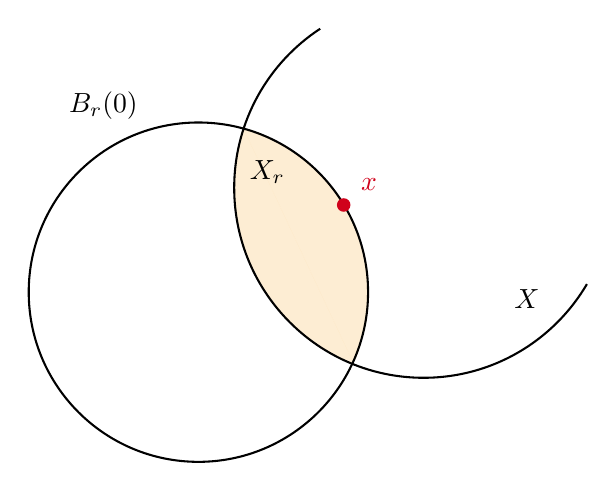
\begin{tikzpicture}[x=0.75pt,y=0.75pt,yscale=-1,xscale=1]
%uncomment if require: \path (0,230); %set diagram left start at 0, and has height of 230

%Curve Lines [id:da2504201730057849] 
\draw [color={rgb, 255:red, 0; green, 0; blue, 0 }  ,draw opacity=0 ][fill={rgb, 255:red, 245; green, 166; blue, 35 }  ,fill opacity=0.2 ]   (292.5,62) .. controls (275.5,114) and (307.5,162) .. (345.5,175) ;


%Curve Lines [id:da9282468110405973] 
\draw [color={rgb, 255:red, 0; green, 0; blue, 0 }  ,draw opacity=0 ][fill={rgb, 255:red, 245; green, 166; blue, 35 }  ,fill opacity=0.2 ]   (345.5,175) .. controls (361.5,140) and (351.5,80) .. (292.5,62) ;



%Shape: Arc [id:dp5893565110889671] 
\draw  [draw opacity=0] (457.94,136.85) .. controls (442.08,163.87) and (412.78,182) .. (379.25,182) .. controls (328.85,182) and (288,141.03) .. (288,90.5) .. controls (288,58.4) and (304.49,30.15) .. (329.44,13.82) -- (379.25,90.5) -- cycle ; \draw   (457.94,136.85) .. controls (442.08,163.87) and (412.78,182) .. (379.25,182) .. controls (328.85,182) and (288,141.03) .. (288,90.5) .. controls (288,58.4) and (304.49,30.15) .. (329.44,13.82) ;
%Shape: Circle [id:dp48240655002847554] 
\draw  [color={rgb, 255:red, 0; green, 0; blue, 0 }  ,draw opacity=1 ] (189,140.75) .. controls (189,95.6) and (225.6,59) .. (270.75,59) .. controls (315.9,59) and (352.5,95.6) .. (352.5,140.75) .. controls (352.5,185.9) and (315.9,222.5) .. (270.75,222.5) .. controls (225.6,222.5) and (189,185.9) .. (189,140.75) -- cycle ;
%Shape: Circle [id:dp47950031726927] 
\draw  [color={rgb, 255:red, 208; green, 2; blue, 27 }  ,draw opacity=1 ][fill={rgb, 255:red, 208; green, 2; blue, 27 }  ,fill opacity=1 ] (338,98.75) .. controls (338,97.23) and (339.23,96) .. (340.75,96) .. controls (342.27,96) and (343.5,97.23) .. (343.5,98.75) .. controls (343.5,100.27) and (342.27,101.5) .. (340.75,101.5) .. controls (339.23,101.5) and (338,100.27) .. (338,98.75) -- cycle ;

% Text Node
\draw (225,51) node [color={rgb, 255:red, 0; green, 0; blue, 0 }  ,opacity=1 ]  {$B_{r}( 0)$};
% Text Node
\draw (353,89) node [color={rgb, 255:red, 208; green, 2; blue, 27 }  ,opacity=1 ]  {$x$};
% Text Node
\draw (429,144) node   {$X$};
% Text Node
\draw (304,83) node [color={rgb, 255:red, 0; green, 0; blue, 0 }  ,opacity=1 ]  {$X_{r}$};


\end{tikzpicture}
